% Created by tikzDevice version 0.6.2-92-0ad2792 on 2013-03-23 23:12:59
% !TEX encoding = UTF-8 Unicode
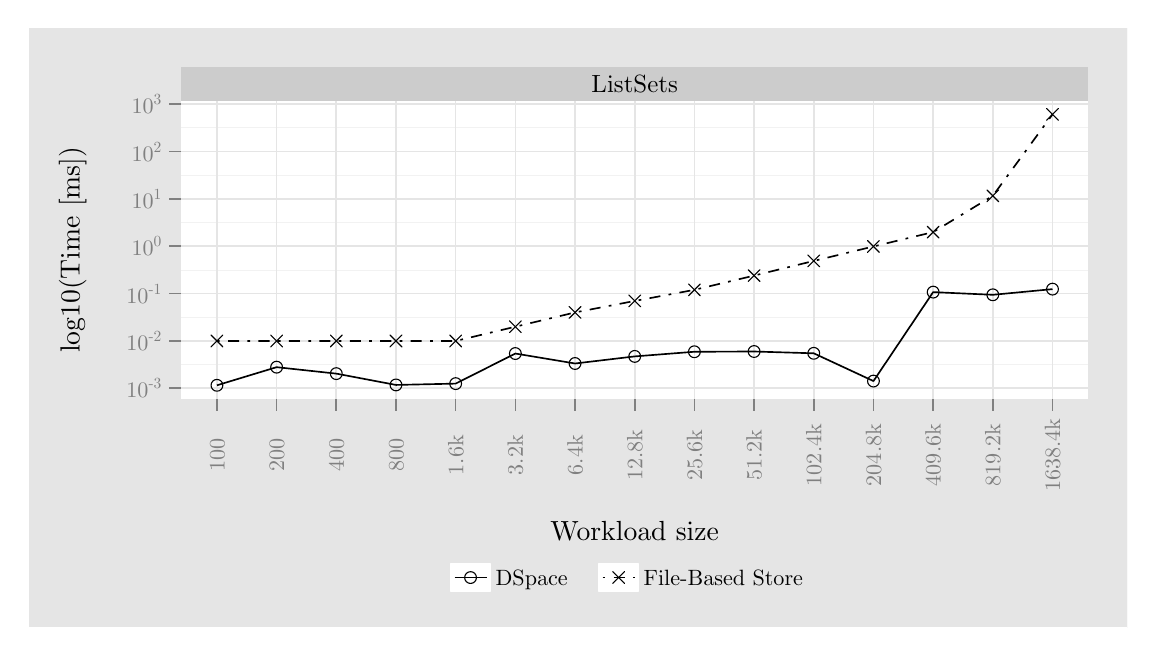
\begin{tikzpicture}[x=1pt,y=1pt]
\definecolor[named]{fillColor}{rgb}{1.00,1.00,1.00}
\path[use as bounding box,fill=fillColor,fill opacity=0.00] (0,0) rectangle (397.48,216.81);
\begin{scope}
\path[clip] (  0.00,  0.00) rectangle (397.48,216.81);
\definecolor[named]{drawColor}{rgb}{1.00,1.00,1.00}
\definecolor[named]{fillColor}{rgb}{0.90,0.90,0.90}

\path[draw=drawColor,line width= 0.6pt,line join=round,line cap=round,fill=fillColor] (  0.00,  0.00) rectangle (397.48,216.81);
\end{scope}
\begin{scope}
\path[clip] ( 55.45, 82.69) rectangle (383.26,190.36);
\definecolor[named]{fillColor}{rgb}{1.00,1.00,1.00}

\path[fill=fillColor] ( 55.45, 82.69) rectangle (383.26,190.36);
\definecolor[named]{drawColor}{rgb}{0.95,0.95,0.95}

\path[draw=drawColor,line width= 0.3pt,line join=round] ( 55.45, 95.05) --
	(383.26, 95.05);

\path[draw=drawColor,line width= 0.3pt,line join=round] ( 55.45,112.16) --
	(383.26,112.16);

\path[draw=drawColor,line width= 0.3pt,line join=round] ( 55.45,129.27) --
	(383.26,129.27);

\path[draw=drawColor,line width= 0.3pt,line join=round] ( 55.45,146.38) --
	(383.26,146.38);

\path[draw=drawColor,line width= 0.3pt,line join=round] ( 55.45,163.49) --
	(383.26,163.49);

\path[draw=drawColor,line width= 0.3pt,line join=round] ( 55.45,180.60) --
	(383.26,180.60);
\definecolor[named]{drawColor}{rgb}{0.90,0.90,0.90}

\path[draw=drawColor,line width= 0.6pt,line join=round] ( 55.45, 86.49) --
	(383.26, 86.49);

\path[draw=drawColor,line width= 0.6pt,line join=round] ( 55.45,103.60) --
	(383.26,103.60);

\path[draw=drawColor,line width= 0.6pt,line join=round] ( 55.45,120.71) --
	(383.26,120.71);

\path[draw=drawColor,line width= 0.6pt,line join=round] ( 55.45,137.82) --
	(383.26,137.82);

\path[draw=drawColor,line width= 0.6pt,line join=round] ( 55.45,154.93) --
	(383.26,154.93);

\path[draw=drawColor,line width= 0.6pt,line join=round] ( 55.45,172.04) --
	(383.26,172.04);

\path[draw=drawColor,line width= 0.6pt,line join=round] ( 55.45,189.15) --
	(383.26,189.15);

\path[draw=drawColor,line width= 0.6pt,line join=round] ( 68.39, 82.69) --
	( 68.39,190.36);

\path[draw=drawColor,line width= 0.6pt,line join=round] ( 89.95, 82.69) --
	( 89.95,190.36);

\path[draw=drawColor,line width= 0.6pt,line join=round] (111.52, 82.69) --
	(111.52,190.36);

\path[draw=drawColor,line width= 0.6pt,line join=round] (133.09, 82.69) --
	(133.09,190.36);

\path[draw=drawColor,line width= 0.6pt,line join=round] (154.65, 82.69) --
	(154.65,190.36);

\path[draw=drawColor,line width= 0.6pt,line join=round] (176.22, 82.69) --
	(176.22,190.36);

\path[draw=drawColor,line width= 0.6pt,line join=round] (197.79, 82.69) --
	(197.79,190.36);

\path[draw=drawColor,line width= 0.6pt,line join=round] (219.35, 82.69) --
	(219.35,190.36);

\path[draw=drawColor,line width= 0.6pt,line join=round] (240.92, 82.69) --
	(240.92,190.36);

\path[draw=drawColor,line width= 0.6pt,line join=round] (262.49, 82.69) --
	(262.49,190.36);

\path[draw=drawColor,line width= 0.6pt,line join=round] (284.05, 82.69) --
	(284.05,190.36);

\path[draw=drawColor,line width= 0.6pt,line join=round] (305.62, 82.69) --
	(305.62,190.36);

\path[draw=drawColor,line width= 0.6pt,line join=round] (327.19, 82.69) --
	(327.19,190.36);

\path[draw=drawColor,line width= 0.6pt,line join=round] (348.75, 82.69) --
	(348.75,190.36);

\path[draw=drawColor,line width= 0.6pt,line join=round] (370.32, 82.69) --
	(370.32,190.36);
\definecolor[named]{drawColor}{rgb}{0.00,0.00,0.00}

\path[draw=drawColor,line width= 0.6pt,line join=round] ( 68.39, 87.58) --
	( 89.95, 94.13) --
	(111.52, 91.80) --
	(133.09, 87.71) --
	(154.65, 88.19) --
	(176.22, 99.06) --
	(197.79, 95.46) --
	(219.35, 98.02) --
	(240.92, 99.70) --
	(262.49, 99.79) --
	(284.05, 99.14) --
	(305.62, 89.11) --
	(327.19,121.25) --
	(348.75,120.28) --
	(370.32,122.33);

\path[draw=drawColor,line width= 0.6pt,dash pattern=on 1pt off 3pt on 4pt off 3pt ,line join=round] ( 68.39,103.60) --
	( 89.95,103.60) --
	(111.52,103.60) --
	(133.09,103.60) --
	(154.65,103.60) --
	(176.22,108.75) --
	(197.79,113.91) --
	(219.35,118.06) --
	(240.92,122.07) --
	(262.49,127.22) --
	(284.05,132.52) --
	(305.62,137.75) --
	(327.19,142.94) --
	(348.75,156.04) --
	(370.32,185.47);

\path[draw=drawColor,line width= 0.4pt,line join=round,line cap=round] ( 68.39, 87.58) circle (  2.13);

\path[draw=drawColor,line width= 0.4pt,line join=round,line cap=round] ( 89.95, 94.13) circle (  2.13);

\path[draw=drawColor,line width= 0.4pt,line join=round,line cap=round] (111.52, 91.80) circle (  2.13);

\path[draw=drawColor,line width= 0.4pt,line join=round,line cap=round] (133.09, 87.71) circle (  2.13);

\path[draw=drawColor,line width= 0.4pt,line join=round,line cap=round] (154.65, 88.19) circle (  2.13);

\path[draw=drawColor,line width= 0.4pt,line join=round,line cap=round] (176.22, 99.06) circle (  2.13);

\path[draw=drawColor,line width= 0.4pt,line join=round,line cap=round] (197.79, 95.46) circle (  2.13);

\path[draw=drawColor,line width= 0.4pt,line join=round,line cap=round] (219.35, 98.02) circle (  2.13);

\path[draw=drawColor,line width= 0.4pt,line join=round,line cap=round] (240.92, 99.70) circle (  2.13);

\path[draw=drawColor,line width= 0.4pt,line join=round,line cap=round] (262.49, 99.79) circle (  2.13);

\path[draw=drawColor,line width= 0.4pt,line join=round,line cap=round] (284.05, 99.14) circle (  2.13);

\path[draw=drawColor,line width= 0.4pt,line join=round,line cap=round] (305.62, 89.11) circle (  2.13);

\path[draw=drawColor,line width= 0.4pt,line join=round,line cap=round] (327.19,121.25) circle (  2.13);

\path[draw=drawColor,line width= 0.4pt,line join=round,line cap=round] (348.75,120.28) circle (  2.13);

\path[draw=drawColor,line width= 0.4pt,line join=round,line cap=round] (370.32,122.33) circle (  2.13);

\path[draw=drawColor,line width= 0.4pt,line join=round,line cap=round,fill=fillColor] ( 66.25,101.47) -- ( 70.52,105.74);

\path[draw=drawColor,line width= 0.4pt,line join=round,line cap=round,fill=fillColor] ( 66.25,105.74) -- ( 70.52,101.47);

\path[draw=drawColor,line width= 0.4pt,line join=round,line cap=round,fill=fillColor] ( 87.82,101.47) -- ( 92.09,105.74);

\path[draw=drawColor,line width= 0.4pt,line join=round,line cap=round,fill=fillColor] ( 87.82,105.74) -- ( 92.09,101.47);

\path[draw=drawColor,line width= 0.4pt,line join=round,line cap=round,fill=fillColor] (109.39,101.47) -- (113.66,105.74);

\path[draw=drawColor,line width= 0.4pt,line join=round,line cap=round,fill=fillColor] (109.39,105.74) -- (113.66,101.47);

\path[draw=drawColor,line width= 0.4pt,line join=round,line cap=round,fill=fillColor] (130.95,101.47) -- (135.22,105.74);

\path[draw=drawColor,line width= 0.4pt,line join=round,line cap=round,fill=fillColor] (130.95,105.74) -- (135.22,101.47);

\path[draw=drawColor,line width= 0.4pt,line join=round,line cap=round,fill=fillColor] (152.52,101.47) -- (156.79,105.74);

\path[draw=drawColor,line width= 0.4pt,line join=round,line cap=round,fill=fillColor] (152.52,105.74) -- (156.79,101.47);

\path[draw=drawColor,line width= 0.4pt,line join=round,line cap=round,fill=fillColor] (174.09,106.62) -- (178.35,110.89);

\path[draw=drawColor,line width= 0.4pt,line join=round,line cap=round,fill=fillColor] (174.09,110.89) -- (178.35,106.62);

\path[draw=drawColor,line width= 0.4pt,line join=round,line cap=round,fill=fillColor] (195.65,111.77) -- (199.92,116.04);

\path[draw=drawColor,line width= 0.4pt,line join=round,line cap=round,fill=fillColor] (195.65,116.04) -- (199.92,111.77);

\path[draw=drawColor,line width= 0.4pt,line join=round,line cap=round,fill=fillColor] (217.22,115.93) -- (221.49,120.20);

\path[draw=drawColor,line width= 0.4pt,line join=round,line cap=round,fill=fillColor] (217.22,120.20) -- (221.49,115.93);

\path[draw=drawColor,line width= 0.4pt,line join=round,line cap=round,fill=fillColor] (238.79,119.93) -- (243.05,124.20);

\path[draw=drawColor,line width= 0.4pt,line join=round,line cap=round,fill=fillColor] (238.79,124.20) -- (243.05,119.93);

\path[draw=drawColor,line width= 0.4pt,line join=round,line cap=round,fill=fillColor] (260.35,125.09) -- (264.62,129.35);

\path[draw=drawColor,line width= 0.4pt,line join=round,line cap=round,fill=fillColor] (260.35,129.35) -- (264.62,125.09);

\path[draw=drawColor,line width= 0.4pt,line join=round,line cap=round,fill=fillColor] (281.92,130.39) -- (286.19,134.66);

\path[draw=drawColor,line width= 0.4pt,line join=round,line cap=round,fill=fillColor] (281.92,134.66) -- (286.19,130.39);

\path[draw=drawColor,line width= 0.4pt,line join=round,line cap=round,fill=fillColor] (303.49,135.61) -- (307.75,139.88);

\path[draw=drawColor,line width= 0.4pt,line join=round,line cap=round,fill=fillColor] (303.49,139.88) -- (307.75,135.61);

\path[draw=drawColor,line width= 0.4pt,line join=round,line cap=round,fill=fillColor] (325.05,140.80) -- (329.32,145.07);

\path[draw=drawColor,line width= 0.4pt,line join=round,line cap=round,fill=fillColor] (325.05,145.07) -- (329.32,140.80);

\path[draw=drawColor,line width= 0.4pt,line join=round,line cap=round,fill=fillColor] (346.62,153.91) -- (350.89,158.18);

\path[draw=drawColor,line width= 0.4pt,line join=round,line cap=round,fill=fillColor] (346.62,158.18) -- (350.89,153.91);

\path[draw=drawColor,line width= 0.4pt,line join=round,line cap=round,fill=fillColor] (368.18,183.33) -- (372.45,187.60);

\path[draw=drawColor,line width= 0.4pt,line join=round,line cap=round,fill=fillColor] (368.18,187.60) -- (372.45,183.33);
\end{scope}
\begin{scope}
\path[clip] (  0.00,  0.00) rectangle (397.48,216.81);
\definecolor[named]{fillColor}{rgb}{0.80,0.80,0.80}

\path[fill=fillColor] ( 55.45,190.36) rectangle (383.26,202.58);
\definecolor[named]{drawColor}{rgb}{0.00,0.00,0.00}

\node[text=drawColor,anchor=base,inner sep=0pt, outer sep=0pt, scale=  0.90] at (219.35,193.37) {ListSets};
\end{scope}
\begin{scope}
\path[clip] (  0.00,  0.00) rectangle (397.48,216.81);
\definecolor[named]{drawColor}{rgb}{0.50,0.50,0.50}

\node[text=drawColor,anchor=base west,inner sep=0pt, outer sep=0pt, scale=  0.80] at ( 35.67, 83.06) {10};

\node[text=drawColor,anchor=base west,inner sep=0pt, outer sep=0pt, scale=  0.56] at ( 43.67, 86.33) {-};

\node[text=drawColor,anchor=base west,inner sep=0pt, outer sep=0pt, scale=  0.56] at ( 45.54, 86.33) {3};

\node[text=drawColor,anchor=base west,inner sep=0pt, outer sep=0pt, scale=  0.80] at ( 35.67,100.17) {10};

\node[text=drawColor,anchor=base west,inner sep=0pt, outer sep=0pt, scale=  0.56] at ( 43.67,103.44) {-};

\node[text=drawColor,anchor=base west,inner sep=0pt, outer sep=0pt, scale=  0.56] at ( 45.54,103.44) {2};

\node[text=drawColor,anchor=base west,inner sep=0pt, outer sep=0pt, scale=  0.80] at ( 35.67,117.28) {10};

\node[text=drawColor,anchor=base west,inner sep=0pt, outer sep=0pt, scale=  0.56] at ( 43.67,120.55) {-};

\node[text=drawColor,anchor=base west,inner sep=0pt, outer sep=0pt, scale=  0.56] at ( 45.54,120.55) {1};

\node[text=drawColor,anchor=base west,inner sep=0pt, outer sep=0pt, scale=  0.80] at ( 37.54,134.39) {10};

\node[text=drawColor,anchor=base west,inner sep=0pt, outer sep=0pt, scale=  0.56] at ( 45.54,137.66) {0};

\node[text=drawColor,anchor=base west,inner sep=0pt, outer sep=0pt, scale=  0.80] at ( 37.54,151.50) {10};

\node[text=drawColor,anchor=base west,inner sep=0pt, outer sep=0pt, scale=  0.56] at ( 45.54,154.77) {1};

\node[text=drawColor,anchor=base west,inner sep=0pt, outer sep=0pt, scale=  0.80] at ( 37.54,168.61) {10};

\node[text=drawColor,anchor=base west,inner sep=0pt, outer sep=0pt, scale=  0.56] at ( 45.54,171.88) {2};

\node[text=drawColor,anchor=base west,inner sep=0pt, outer sep=0pt, scale=  0.80] at ( 37.54,185.72) {10};

\node[text=drawColor,anchor=base west,inner sep=0pt, outer sep=0pt, scale=  0.56] at ( 45.54,188.99) {3};
\end{scope}
\begin{scope}
\path[clip] (  0.00,  0.00) rectangle (397.48,216.81);
\definecolor[named]{drawColor}{rgb}{0.50,0.50,0.50}

\path[draw=drawColor,line width= 0.6pt,line join=round] ( 51.18, 86.49) --
	( 55.45, 86.49);

\path[draw=drawColor,line width= 0.6pt,line join=round] ( 51.18,103.60) --
	( 55.45,103.60);

\path[draw=drawColor,line width= 0.6pt,line join=round] ( 51.18,120.71) --
	( 55.45,120.71);

\path[draw=drawColor,line width= 0.6pt,line join=round] ( 51.18,137.82) --
	( 55.45,137.82);

\path[draw=drawColor,line width= 0.6pt,line join=round] ( 51.18,154.93) --
	( 55.45,154.93);

\path[draw=drawColor,line width= 0.6pt,line join=round] ( 51.18,172.04) --
	( 55.45,172.04);

\path[draw=drawColor,line width= 0.6pt,line join=round] ( 51.18,189.15) --
	( 55.45,189.15);
\end{scope}
\begin{scope}
\path[clip] (  0.00,  0.00) rectangle (397.48,216.81);
\definecolor[named]{drawColor}{rgb}{0.50,0.50,0.50}

\path[draw=drawColor,line width= 0.6pt,line join=round] ( 68.39, 78.42) --
	( 68.39, 82.69);

\path[draw=drawColor,line width= 0.6pt,line join=round] ( 89.95, 78.42) --
	( 89.95, 82.69);

\path[draw=drawColor,line width= 0.6pt,line join=round] (111.52, 78.42) --
	(111.52, 82.69);

\path[draw=drawColor,line width= 0.6pt,line join=round] (133.09, 78.42) --
	(133.09, 82.69);

\path[draw=drawColor,line width= 0.6pt,line join=round] (154.65, 78.42) --
	(154.65, 82.69);

\path[draw=drawColor,line width= 0.6pt,line join=round] (176.22, 78.42) --
	(176.22, 82.69);

\path[draw=drawColor,line width= 0.6pt,line join=round] (197.79, 78.42) --
	(197.79, 82.69);

\path[draw=drawColor,line width= 0.6pt,line join=round] (219.35, 78.42) --
	(219.35, 82.69);

\path[draw=drawColor,line width= 0.6pt,line join=round] (240.92, 78.42) --
	(240.92, 82.69);

\path[draw=drawColor,line width= 0.6pt,line join=round] (262.49, 78.42) --
	(262.49, 82.69);

\path[draw=drawColor,line width= 0.6pt,line join=round] (284.05, 78.42) --
	(284.05, 82.69);

\path[draw=drawColor,line width= 0.6pt,line join=round] (305.62, 78.42) --
	(305.62, 82.69);

\path[draw=drawColor,line width= 0.6pt,line join=round] (327.19, 78.42) --
	(327.19, 82.69);

\path[draw=drawColor,line width= 0.6pt,line join=round] (348.75, 78.42) --
	(348.75, 82.69);

\path[draw=drawColor,line width= 0.6pt,line join=round] (370.32, 78.42) --
	(370.32, 82.69);
\end{scope}
\begin{scope}
\path[clip] (  0.00,  0.00) rectangle (397.48,216.81);
\definecolor[named]{drawColor}{rgb}{0.50,0.50,0.50}

\node[text=drawColor,rotate= 90.00,anchor=base,inner sep=0pt, outer sep=0pt, scale=  0.80] at ( 71.14, 62.36) {100};

\node[text=drawColor,rotate= 90.00,anchor=base,inner sep=0pt, outer sep=0pt, scale=  0.80] at ( 92.71, 62.36) {200};

\node[text=drawColor,rotate= 90.00,anchor=base,inner sep=0pt, outer sep=0pt, scale=  0.80] at (114.28, 62.36) {400};

\node[text=drawColor,rotate= 90.00,anchor=base,inner sep=0pt, outer sep=0pt, scale=  0.80] at (135.84, 62.36) {800};

\node[text=drawColor,rotate= 90.00,anchor=base,inner sep=0pt, outer sep=0pt, scale=  0.80] at (157.41, 62.36) {1.6k};

\node[text=drawColor,rotate= 90.00,anchor=base,inner sep=0pt, outer sep=0pt, scale=  0.80] at (178.98, 62.36) {3.2k};

\node[text=drawColor,rotate= 90.00,anchor=base,inner sep=0pt, outer sep=0pt, scale=  0.80] at (200.54, 62.36) {6.4k};

\node[text=drawColor,rotate= 90.00,anchor=base,inner sep=0pt, outer sep=0pt, scale=  0.80] at (222.11, 62.36) {12.8k};

\node[text=drawColor,rotate= 90.00,anchor=base,inner sep=0pt, outer sep=0pt, scale=  0.80] at (243.67, 62.36) {25.6k};

\node[text=drawColor,rotate= 90.00,anchor=base,inner sep=0pt, outer sep=0pt, scale=  0.80] at (265.24, 62.36) {51.2k};

\node[text=drawColor,rotate= 90.00,anchor=base,inner sep=0pt, outer sep=0pt, scale=  0.80] at (286.81, 62.36) {102.4k};

\node[text=drawColor,rotate= 90.00,anchor=base,inner sep=0pt, outer sep=0pt, scale=  0.80] at (308.37, 62.36) {204.8k};

\node[text=drawColor,rotate= 90.00,anchor=base,inner sep=0pt, outer sep=0pt, scale=  0.80] at (329.94, 62.36) {409.6k};

\node[text=drawColor,rotate= 90.00,anchor=base,inner sep=0pt, outer sep=0pt, scale=  0.80] at (351.51, 62.36) {819.2k};

\node[text=drawColor,rotate= 90.00,anchor=base,inner sep=0pt, outer sep=0pt, scale=  0.80] at (373.07, 62.36) {1638.4k};
\end{scope}
\begin{scope}
\path[clip] (  0.00,  0.00) rectangle (397.48,216.81);
\definecolor[named]{drawColor}{rgb}{0.00,0.00,0.00}

\node[text=drawColor,anchor=base,inner sep=0pt, outer sep=0pt, scale=  1.00] at (219.35, 31.41) {Workload size};
\end{scope}
\begin{scope}
\path[clip] (  0.00,  0.00) rectangle (397.48,216.81);
\definecolor[named]{drawColor}{rgb}{0.00,0.00,0.00}

\node[text=drawColor,rotate= 90.00,anchor=base,inner sep=0pt, outer sep=0pt, scale=  1.00] at ( 18.80,136.53) {log10(Time [ms])};
\end{scope}
\begin{scope}
\path[clip] (  0.00,  0.00) rectangle (397.48,216.81);
\definecolor[named]{fillColor}{rgb}{0.90,0.90,0.90}

\path[fill=fillColor] (144.93,  8.87) rectangle (293.78, 27.36);
\end{scope}
\begin{scope}
\path[clip] (  0.00,  0.00) rectangle (397.48,216.81);
\definecolor[named]{drawColor}{rgb}{1.00,1.00,1.00}
\definecolor[named]{fillColor}{rgb}{1.00,1.00,1.00}

\path[draw=drawColor,line width= 0.6pt,line join=round,line cap=round,fill=fillColor] (152.81, 13.14) rectangle (167.26, 23.09);
\end{scope}
\begin{scope}
\path[clip] (  0.00,  0.00) rectangle (397.48,216.81);
\definecolor[named]{drawColor}{rgb}{0.00,0.00,0.00}

\path[draw=drawColor,line width= 0.6pt,line join=round] (154.25, 18.11) -- (165.82, 18.11);
\end{scope}
\begin{scope}
\path[clip] (  0.00,  0.00) rectangle (397.48,216.81);
\definecolor[named]{drawColor}{rgb}{0.00,0.00,0.00}

\path[draw=drawColor,line width= 0.4pt,line join=round,line cap=round] (160.03, 18.11) circle (  2.13);
\end{scope}
\begin{scope}
\path[clip] (  0.00,  0.00) rectangle (397.48,216.81);
\definecolor[named]{drawColor}{rgb}{1.00,1.00,1.00}
\definecolor[named]{fillColor}{rgb}{1.00,1.00,1.00}

\path[draw=drawColor,line width= 0.6pt,line join=round,line cap=round,fill=fillColor] (206.31, 13.14) rectangle (220.77, 23.09);
\end{scope}
\begin{scope}
\path[clip] (  0.00,  0.00) rectangle (397.48,216.81);
\definecolor[named]{drawColor}{rgb}{0.00,0.00,0.00}

\path[draw=drawColor,line width= 0.6pt,dash pattern=on 1pt off 3pt on 4pt off 3pt ,line join=round] (207.76, 18.11) -- (219.32, 18.11);
\end{scope}
\begin{scope}
\path[clip] (  0.00,  0.00) rectangle (397.48,216.81);
\definecolor[named]{drawColor}{rgb}{0.00,0.00,0.00}
\definecolor[named]{fillColor}{rgb}{1.00,1.00,1.00}

\path[draw=drawColor,line width= 0.4pt,line join=round,line cap=round,fill=fillColor] (211.41, 15.98) -- (215.67, 20.25);

\path[draw=drawColor,line width= 0.4pt,line join=round,line cap=round,fill=fillColor] (211.41, 20.25) -- (215.67, 15.98);
\end{scope}
\begin{scope}
\path[clip] (  0.00,  0.00) rectangle (397.48,216.81);
\definecolor[named]{drawColor}{rgb}{0.00,0.00,0.00}

\node[text=drawColor,anchor=base west,inner sep=0pt, outer sep=0pt, scale=  0.80] at (169.07, 15.36) {DSpace $\;\;\;$};
\end{scope}
\begin{scope}
\path[clip] (  0.00,  0.00) rectangle (397.48,216.81);
\definecolor[named]{drawColor}{rgb}{0.00,0.00,0.00}

\node[text=drawColor,anchor=base west,inner sep=0pt, outer sep=0pt, scale=  0.80] at (222.57, 15.36) {File-Based Store $\;\;\;$};
\end{scope}
\end{tikzpicture}
